\documentclass[a4paper,12pt]{article}
\usepackage[T1]{fontenc}
\usepackage[u  tf8]{inputenc}
\usepackage{mathtools}
\usepackage{mathrsfs}
\usepackage{bm}
\usepackage{amsfonts}
\usepackage[dvipsnames]{xcolor}
% \usepackage{cleveref}
\usepackage[normalem]{ulem}
\usepackage{graphicx}
\usepackage{fullpage}
\usepackage[margin=1in]{geometry}
\usepackage{natbib}
\usepackage{amsmath}
%\usepackage{float}
%\usepackage{subcaption}
%\usepackage{multirow} 
\usepackage[colorlinks = true,urlcolor=blue]{hyperref}
%\usepackage{bibunits}
%\usepackage{csvsimple}
%\usepackage[superscript,biblabel]{cite}
\usepackage{verbatim}
\usepackage{graphicx}
\graphicspath{ {final_images/} }
\usepackage{subfig}
% \usepackage{subcaption}
\usepackage{geometry}
\usepackage{dirtytalk}

\newcommand{\jb}[1]{{\color{blue} (#1)} }
\begin{document}

\title{\vspace{-2cm}
  The Effect of Directional Dominance on Additive Effect Sizes
}
\author{\normalsize{Kyelee Fitts, Jeremy Berg, Yuval Simons, Guy
    Sella \\
  \small{Systems Biology Department}}}
\date{\normalsize{\today}}
\maketitle



\subsection*{Abstract}
The averge effect size $\alpha$ is the estimated effect size for an
allele for a polygenic trait. These effect sizes are estimated using
Genome-Wide Association Studies, and we can estimate signals of natural
selection for polygenic traits by weighting by $\alpha$ in statistical
tests for polygenic adaptation. However, in the presence of
directional dominance, we hypothesized that such statistical tests
could be biased. For example, alleles which are systematically
dominant and have increased in frequency in the recent past will have
deflated average effect sizes, and vice versa. Simulations of the test
statistic $Q_x$ used to detect polygenic adaptation, expanded to
account for dominance effects, show that the effect that directional
dominance has on the statistic is to shift the distribution to the
right. Furthermore, directional dominance causes $\alpha$ to
systematically stretch or shrink genetic value over generations,
further pointing to inflations of deflations of $\alpha$ in accordance
with directional dominance. Preliminary investigations of the UK
Biobank data for height show that height displays both polygenic
adaptation and directional dominance.


\subsection*{Introduction}

The diversity of life on Earth is due in large part to the
adaptation of organisms to their varying environments. We now know that
adaptation has a large genetic basis. Thus, understanding how and why such
genetic variation occurs is a major goal of evolutionary
biology. Quantifying genetic adaptation is an important aim of population
geneticists, and to this end finding methods to detect signals of
selection within the genome is of particular interest. Change in the
mean phenotype of a population over time can be attributed to many causes including genetic
drift or gene flow, so detecting signals of selection in
particular is no trivial task.

\begin{comment}
  So I might frame this next paragraph differently. I might suggest a bit more expanded intro,
  and then a slightly different tack after that. Something like:

  Until recently, population genetic methods to detect adaptation have been limited to
  identifying individual loci which have experienced implausibly large allele frequency changes
  in the recent past, a signal of recent and strong natural selection. However, when phenotypes
  are highly polygenic (i.e. many genes are responsible for phentoypic variations, the response
  to selection gets spread out among many loci, such that no individual allele will look unusual
  against the background of genetic drift. Our understanding of the genetic basis of adaptation
  may therefore be substantially biased toward large effect alleles....
\end{comment}

Until recently, the population genetic methods to detect recent adaptation have been limited to
large-effect alleles by finding individual loci with significant
allele frequency changes in the recent past-- this is an indication of
strong, recent national selection. However, many phenotypes of interest
are affected by many different loci across the genome. These are known
as polygenic traits. When natural selection occurs with polygenic
traits, the signal of selection get spread out over many loci, such
that no individual loci displays large frequency changes against the
background of genetic drift.  Understanding
how to find signals of natural selection for such polygenic traits has been
the subject of much study in recent years.

Increased computational capabilities have given us the tools to be able to evaluate the effects
of many thousands of loci on a trait, allowing us to evaluate
selection in highly polygenic traits, such as height. One of the most
important tools developed are Genome-Wide Association Studies (GWAS)
which determine which loci across the genome have significant effects
on a certain polygenic trait \cite{gwasoverview} and what the average
effect sizes of those loci are. GWAS works by
estimating a linear regression based on the following model \cite{gwas}:

  \begin{align}
    \vec{Y} = \mu + \alpha \vec{g} + \vec{\epsilon}
  \end{align}

Where $\vec{Y}$ is a vector of the measurements of the phenotype of
interest over a population of genetically unrelated individuals,
$\vec{g}$ is a vector of the genotypes of each individual, $\mu$ is
the mean phenotype in the sample, and $\alpha$ is the average
effect in the sample of switching the allele with the
other allele at the given locus. $\vec{\epsilon}$ is the vector of
error terms for each individual. GWAS performs a linear regression
using this model, where under the null model (that the
allele does not contribute to polygenic selection and is only subject
to drift) $\alpha = 0$. 

Turchin et al. \cite{heightselection} were the first to show how this
GWAS data could be used to detect signals of selection in polygenic
traits. The idea is to look for coordinated shifts in frequency over
many different loci associated with a polygenic trait to find
statistically significant changes in allele frequency that are
unlikely to have been caused by drift alone. These tests depend on the
fact that under drift (the null hypothesis), the effect sizes $\alpha$
and the allele frequencies of the alleles are independent. However, we hypothesize that this assumption is violated
under certain conditions, namely directional dominance. 

\begin{comment}
  Recent work has relied on genome-wide association studies (GWAS) as a way past this obstacle.
  The aim of GWAS is to identify individual sites that are responsible for contributing to genetic
  variation in a polygenic phenotype. This is done by performing the linear regression
  \begin{align}
    \vec{Y} = \mu + \alpha \vec{g} + \vec{\epsilon}
  \end{align}
  where $\vec{Y}$ is a vector of phenotypic measurements for a large cohort of geneticall unrelated individuals,
  $\vec{g}$ is a vector of measured genotypes, $\mu$ and $\vec{\epsilon}$ are the mean phenotype in the sample
  and the vector of residuals respectively, and $\alpha$ is the average effect on the phenotype of
  substituting one allele for the other at the site in question. GWAS works by performing a null hypothesis
  significance test of this model (where the null hypothesis is that $\alpha = 0$) for each site in the genome,
  typically using a strict significance cutoff of $p<5\times 10^{-8}$. The result is a list of loci
  putatively associated with the trait, as well as estimates of their effect sizes $\alpha$.

  Turchin et al (2012) were the first to show how GWAS data could be used to detect signals of selection on
  polygenic traits. Crucially, gives us an annotation of which sites throughout the genome affect a
  particular trait, and tells us which allele increases the trait an which decreases it. With these annotations,
  the limitation outlined above can be overcoming by looking for subtle but coordinated shifts in
  frequency across many trait associated alleles that would be extremely unlikely to arise under
  genetic drift alone.

  (then you can explain about the fact that under drift we expect no association between the $\alpha$
  and the direction of allele frequency change, and that tests of polygenic adaptation are therefore
  tests for whether such an association exists. This then gives you a segue into the fact that all of the above
  assumes that there is no dominance, but that if there is dominance (and particularly if there's directional
  dominance) then the $\alpha$s estimated in GWAS depend on allele frequency, and then our assumptions about
  independence of $\alpha$ and the recent direction of allele frequency change no longer hold. At that point
  the project is pretty well motivated, and you can move on to theory/methods.)
  
\end{comment}

\begin{comment}
We can express the polygenic phenotype of individuals in a population
as the weighted sum of genotypes with additive effect sizes
$\alpha$. This generalizes to population means, where the mean
population phenotype is the weighted sum of effect sizes and frequency
of the allele ($p$) at each significant locus ($l$). \cite{gillespie}

\begin{equation}
  \sum_l{\alpha_lp_l}
\end{equation}

The additive effect size, then, is key to relating the genotypes of
the many loci contributing to the phenotype of interest with the
phenotype itself-- as shown below, it also plays a key role in statistical tests for
polygenic adaptaion. Understanding how $\alpha$ can be
affected by other factors is essential for ensuring that these
statistical tests remain as unbiased as possible.
\end{comment}

Dominance in population genetics refers to when the effect of one
allele depends on the presence of another allele at the locus. We can account for
the effect of dominance in the effect size by parametrizing $\alpha$
in terms of the homozygous effect size (A), or effect size of the most frequent homozygote, and the
dominance deviation (D), which is the difference in effect size for the heterozygote
deviating from $\frac{1}{2}$ of the homozygous effect size \cite{gillespie}:

\begin{equation}  
  \alpha_\ell = \frac{1}{2} A_\ell + D_\ell\left(1-2p_{1\ell}\right).
  \label{alpha}
\end{equation}

In particular, directional dominance is when alleles with a postive effect
size on the trait are systematically dominant and alleles with a
negative effect size on the trait are systematically recessive or vice
versa (i.e., dominant alleles have a negative effect or recessive have
a positive effect). In terms of \eqref{alpha}, this means that the
average D over all loci is different from zero. Specifically, while
many alleles contributing to a trait will have nonzero dominance
deviations, on expectation these will be zero. However, directional
dominance occurs when the dominance deviations over many alleles is on
expectation nonzero.

We hypothesized that directional dominance is problematic in tests of polygenic adaptation
because the effect size we estimate in the presence of directional
dominance depends on how the allele frequency $p$ has changed in the
recent past. In particular, recessive alleles which have decreased in frequency
in the recent past will tend to have larger effect sizes, as shown in
Figure 1 in the supplement. Notice that when there is no dominance,
$\alpha$ is constant, but in the presence of directional dominance
(average $D\neq0$) for alleles with lower frequency will have a higher
effect size. 

Given the hypothesized effect that directional dominance has on
$\alpha$, we suspect that directional dominance will bias statistical
tests of polygenic adaptation. We give a short overview of some
central ideas in tests for selection below before introducing the test
statistic for detecting polygenic adaptation.


\begin{comment}so I think you're using the following to sort of
  outline the basic idea of the tests. I'm not sure if this extended
  history/background about $F_{ST}$ and $Q_{ST}$ is totally
  necessary. It's all accurate, but it not clear that it really helps
  inform the reader about what's coming below.
\end{comment}

Wright first introduced the parameter $F_{st}$ as a measure comparing
the genetic variation of an allele at a specific site in a subpopulation to that of the entire population
\cite{Fst}. Lewontin and Krakauer, using this parameter developed a
novel statistical test based on the fact
that under no selection, the expected $F_{st}$ at a given site will be the same
as the population $F_{st}$. Further, they concluded that the
distribution of $F_{st}$ across all sites will be chi-squared
$F_{st}$ \cite{firstseltest}. The natural conclusion is that sites
with statistically different $F_{st}$ values are candidates for loci
that have been acted upon by selection. These conclusions were extended by Spitze, who coined the
parameter $Q_{st}$ as a measure of how the variation of all loci
contributing to a phenotype of a subpopulation compares to that of the entire
population \cite{Qst}. Essentially, $Q_{st}$ is analogous to $F_{st}$,
except that instead of looking at the variation of one allele at a
locus, it measures the ratio of the variation of all loci contributing to a
phenotype within a subpopulation to that of the entire population. These early tests for selection utilized the ratio
$\frac{Q_{st}}{F_{st}}$ as a test statistic for detecting signals of
selection, where $F_{st} = Q_{st}$ is the null model, where no
selection occurs.

Much later, based on these central ideas as well as Turchin's test \cite{heightselection} to test
for selection in polygenic traits, Berg and Coop introduced a comprehensive test statistic,
called $Q_x$, to test for selection in polygenic traits \cite{berg}. This statistic depends on $F_{st}$ and
a generalized analogy to $Q_{st}$, expressed in terms of $\alpha$ and
the allele frequencies $p$ over loci $l$ and $l'$, summed over
populations $m$. $V_a$ is the additive genetic variance of the entire
population, and $\overline{p}_l$ is the mean frequency.

\begin{equation} \label{Qxraw}
  Q_X = \frac{1}{V_A F_{ST}} \sum_{m=1}^M \sum_{\ell=1}^L \sum_{\ell\prime=1}^L \alpha_{\ell} \alpha_{\ell^{\prime}}\left(p_{m\ell} - \overline{p}_\ell \right)\left(p_{m \ell\prime} - \overline{p}_{\ell\prime}\right)
\end{equation}


The distribution of this statistic is expected to be chi-squared. Notice that the additive effect size $\alpha$ is the weighting factor for loci in the
expression for $Q_x$. 

In the presence of directional dominance, we hypothesized a bias in
tests for polygenic adaptation that depends on $\alpha$. For example, alleles which are dominant and which have recently increased in
frequency (large p, positive D, for positive A) will tend to have smaller effect sizes, while
alleles which are dominant which have recently decreased in frequency
(small p, negative D, for positive A) will tend to have larger effect sizes. In the
latter case, the test for polygenic selection advanced by Berg and Coop
\eqref{Qxraw} will tend to make false positive judgements for
selection, because the statistic will be calculated over alleles which
do not actually increase the effect size.


\begin{comment}
  it's not just that height has many significantly associated alleles, but that it
  shows evidence of polygenic adaptation. The fact that it exhibits evidence for both polygenic adaptation
  and directional dominance is what's potentially worrying. Making sure you drive that home right at the end of
  the intro is key I think, because then you will have given your reader all the theory/conceptual tools to
  understand the scenario in which a problem may exist, and then cited data to convince them that a problem indeed DOES exist.
\end{comment}
Height is one polygenic trait with many well-defined signficant
alleles via GWAS \cite{heightselection} that also shows evidence of polygenic selection. It has also been shown to exhibit
directional dominance \cite{heightdirectdom}. In otherwords, we
suspect that the non-independence between allele frequency and effect
size caused by directional dominance will cause tests of polygenic
adaptation to over or underestimate signals of polygenic selection. We aim to quantify the
hypothesized bias, first with simulated populations, then with height genotype data from the UK Biobank.



\subsection*{Theory/Methods}



Using the expression for the test statistic $Q_x$ \eqref{Qxraw}, we
can substitute the expression for $\alpha$ \eqref{alpha} and manipulate
the expression algebraically to derive the following expansion for the
test statistic, in terms of the homozygous effect (A)  and the dominance
deviation (D):

\begin{equation}
  \begin{split}
  \sum^L_{l=1}( \frac{1}{2}A_l(p_{1l}-\epsilon_l))^2+\sum^L_{l=1}\sum^L_{
    l \neq l'}(\frac{1}{4}A_l(p_{1l}-\epsilon_{l})A_{l'}(p_{1l'}-\epsilon_{l'}))
  \\
  +\sum^L_{l=1}A_lD_l(1-2p_{1l})(p_{1l}-\epsilon_l)^2 +
  \sum^L_{l=1}\sum^L_{l \neq
    l'}(\frac{1}{2}A_lD_{l'}(1-2_{p1l'})(p_{1l}-\epsilon_l)(p_{1l'}-\epsilon_{l'}) \\
  + \frac{1}{2}D_lA_{l'}(1-2_{p1l})(p_{1l}-\epsilon_l)(p_{1l'}-\epsilon_{l'})) \\
   + \sum^L_{l=1} (D_l(1-2p_l)(p_{1l}-\epsilon_{1}))^2
   + \sum^L_{l=1}\sum^L_{l \neq
     l'}D_{l}(1-2p_{l})(p_{1l}-\epsilon_{1})D_{l'}(1-2p_{l'})(p_{1l'}-\epsilon_{l'}) \label{expansion}
  \end{split}
\end{equation}

We can loosly consider the single summation terms to be variances
corresponding to the expansion of additive effects multiplied by
additive effects, additive times dominance, and dominance times
dominance, and the double summation terms as covariances of these
quantities. We expect the inflation of the test statistic due to
dominance effects to come from the last two terms. Note that when
dominance is not present ($D=0$) the expansion reduces to the
expression Berg and Coop present when $\alpha$ is treated as a constant
\cite{berg}.

Using this expansion, we have created simulations to characterize our
hypothesized dominance bias. We used simulated populations
under a couple of assumptions: first, that the values of the dominance
deviations and homozygous effects are constant throughout the
population. While this is not true in general, we expect that the
distributions of these parameters are roughly normal
\cite{normaldist}, and noise around the expected values of the
dominance deviations or homozygous effects should not affect the distribution of the test statistic too
much. Second, that $F_{st}$ for these simulated approximations
can be roughly estimated by the number of generations elapsed over the
population size \cite{Fstest}. Third, that the distribution of allele frequencies after
one generation can be approximated by a normal distribution centered
at the ancestral frequency with variance
$F_{st}*\epsilon*(1-\epsilon)$ where $\epsilon$ is the ancestral
frequency \cite{gillespie}.

All simulations were performed in R. 

\subsection*{Results/Discussion}
Simulations of the expansion \eqref{expansion} were performed with
population size $10000$ over 100 generations, starting at an ancestral
frequency of 0.5, an homozygous effect size of 0.5, and a dominance
deviation value of 0 (Figure 2). The distribution of $Q_x$ was simulated under
these conditions for 1000 replicates. The distribution was roughly
chi-squared, as expected, with mean of 0.99 and variance of
2.2. Adding directional dominance effects to simulation led to a shift of the
distribution, as shown in Figure 3.

To further explore this shift, we plotted the expected cumulative
distribution function of the distribution of the test statistic over
several different dominance deviation values. Figure 4 shows that with
no dominance, the cdf of the statistic is very close to the expected
cdf of a chi-squared distributed function (in red), with mean 1 and variance 2
(as expected for a statistic taken over one population). For dominance
deviations greater than 0 (Figure 5 shows the expected cdf of a
statistic with dominance deviation of 0.5), the distribution is
strongly shifted to the right. This observation is taken further in
Figure 6, where we plot the proportion of the test statistic over the
threshold of the statistic such that p = 0.05. In otherwords, we plot the
proportion of false positives for the test statistic in the presence
of directional dominance. For dominance deviation
values of 0, this proportion is very close to 0.05. However, as
dominance effects increase, there is a corresponding increase in the
proportion of the statistic over this threshold. Notice that as the
dominance deviation approaches 1 (complete dominance), almost all of
the values of $Q_x$ are  over the expected threshold.

Next, we were interested in seeing how the effect of dominance affects
the average effect size over time. We simulated the frequency of an
allele over 1000 generations under the Normal approximation to drift
both without dominance (Figure 7) and with a dominance value of 0.2
(Figure 8), replicating this simulation 10000 times, representing 10000
simulated populations. The red line shows the average allele frequency
over time. As expected for no dominance the average allele frequency
stays at 0.5, or the ancestral allele frequency, because alleles
are equally likely to be fixed or lost among many populations in this
case. Interestingly, for a dominance deviation of 0.2, the average allele
frequency also appears to stay very close to the ancestral frequency,
indicating that for this low of a dominance deviation it is difficult
to qualitatively distinguish between the proportion of populations
that fix the allele and the proportion of populations for which the
allele is lost.

However, by plotting the genetic value (allele frequency multiplied by
average effect size) of a simulated allele over time, we expect to see
that dominance will have a nontrivial effect on the trajectory of the
average genetic value. This is because while there is still on average
an even split between populations that fix the allele and populations
that lose it, the multiplication of the average effect will have the
effect of \say{stretching} the genetic value of alleles that have
recently increased in frequency in the case of negative dominance
deviations (Figure 10) or decreased in frequency in the case of
positive dominance deviations (Figure 11), with a corresponding
shrinkage in the opposite direction. Indeed, we see that the
average genetic value (red line). Figure 9 shows the genetic value
over time of populations with no dominance, which as expected, with no
stretching or shrinking of the genetic value in either direction.

This last plot is particularly interesting because it shows that in
the presence of directional dominance, the stretching and shrinking
effect of $\alpha$ has the potential to skew the genetic value of the
allele in question, meaning not only that GWAS is more likely to
choose these alleles as significant for selection, but also that when
these alleles are used in the test statistic $Q_x$, their contribution
will be inflated or deflated, because the average effect is what
weighs alleles in the statistic.

Finally, in order to look for the effects of directional dominance on
the average effect size in alpha, we wanted to show that height is one
polygenic trait that shows signals of directional dominance. To this
end, taking GWAS data from the UK Biobank, we created a qq plot of the
dominance deviation p-values, choosing SNPs that were 
most significant ($p <= 10^{-8}$) p-values for the average effect size
over all chromosomes. Figure 12 shows that the p-values are skewed--
in otherwords, we see that for a large number of significant sites,
the dominance deviation p-values are not distributed as we would
expect, indicating that there are signs of dominance in height.

Furthermore, we verified that height shows signals of directional
dominance in particular by bootstrapping the dominance deviation
values to see if on average they are nonzero across all
significant loci (Figure 13). We chose alleles with average effect size p-value
$<= 10^{-8}$ and used sampled the most significant alleles within
blocks of approximately independent alleles in the genome (to account
for linkage effects). With 10000 replicates, we found a mean of
$7.9*10^{-4}$, which suggests that dominance deviations are at least
slightly nonzero and the height displays directional dominance.  

\subsection*{Conclusion}
These simulated results and the preliminary UKBiobank verification of
directional dominance in height suggest that, as hypothesized, the
effect of directional dominance on the average effect size is
nontrivial and in fact could result in false positives or negatives in
the statistical tests for polygenic adaptation. Although we have no
reason to suspect this effect is very large, as dominance
itself does not an particularly large effect on polygenic traits in
general, quantifying this effect in height could open many potential
avenues of research in understanding how tests for polygenic
adaptation could be biased.

Next steps for this project in particular are delving into the
UKBiobank data in earnest, performing an in-house GWAS and
substracting dominance deviation and homozygous effect size data from
alleles that show signs of directional dominance.

\subsection*{Acknowledgements}
Thank you to Jeremy Berg, my mentor in the Sella Lab, as well as to
Yuval Simons, who initially proposed this project, and Guy Sella, my
PI. Thank you also to Hakhamanesh Mostafavi for providing GWAS data
for the preliminary analysis of the UK Biobank data. 


\pagebreak
\bibliography{works_cited}
\bibliographystyle{plain}


 \newgeometry{left=0.5in, right=0.5in, bottom=0.2in, top=0.5in}
 \begin{table}[ht]
 \caption*{Supplement}
 \centering
 \begin{tabular}{ p{9cm}p{9cm} }
 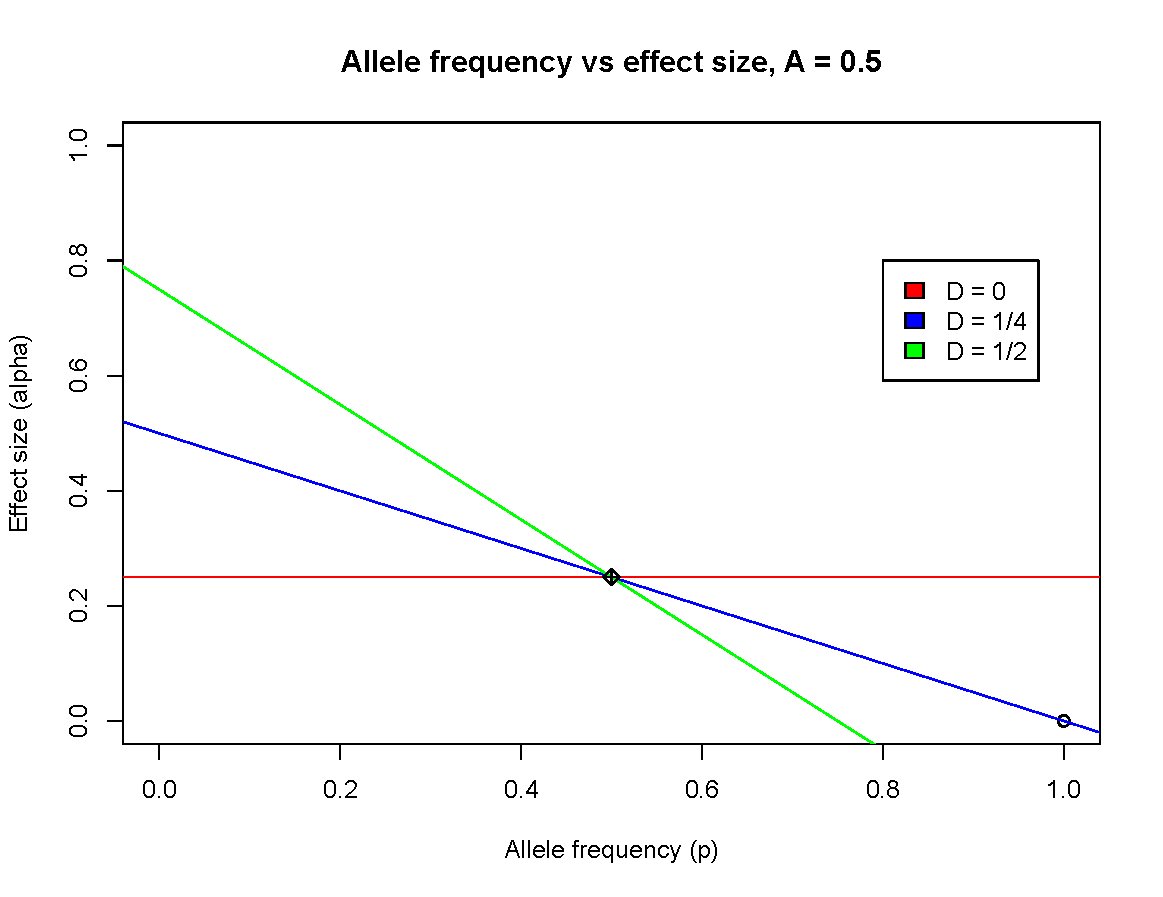
\includegraphics[width=80mm]{alpha} \caption*{Fig. 1: Effect sizes for various
    dominance deviation values under directional dominance}
    &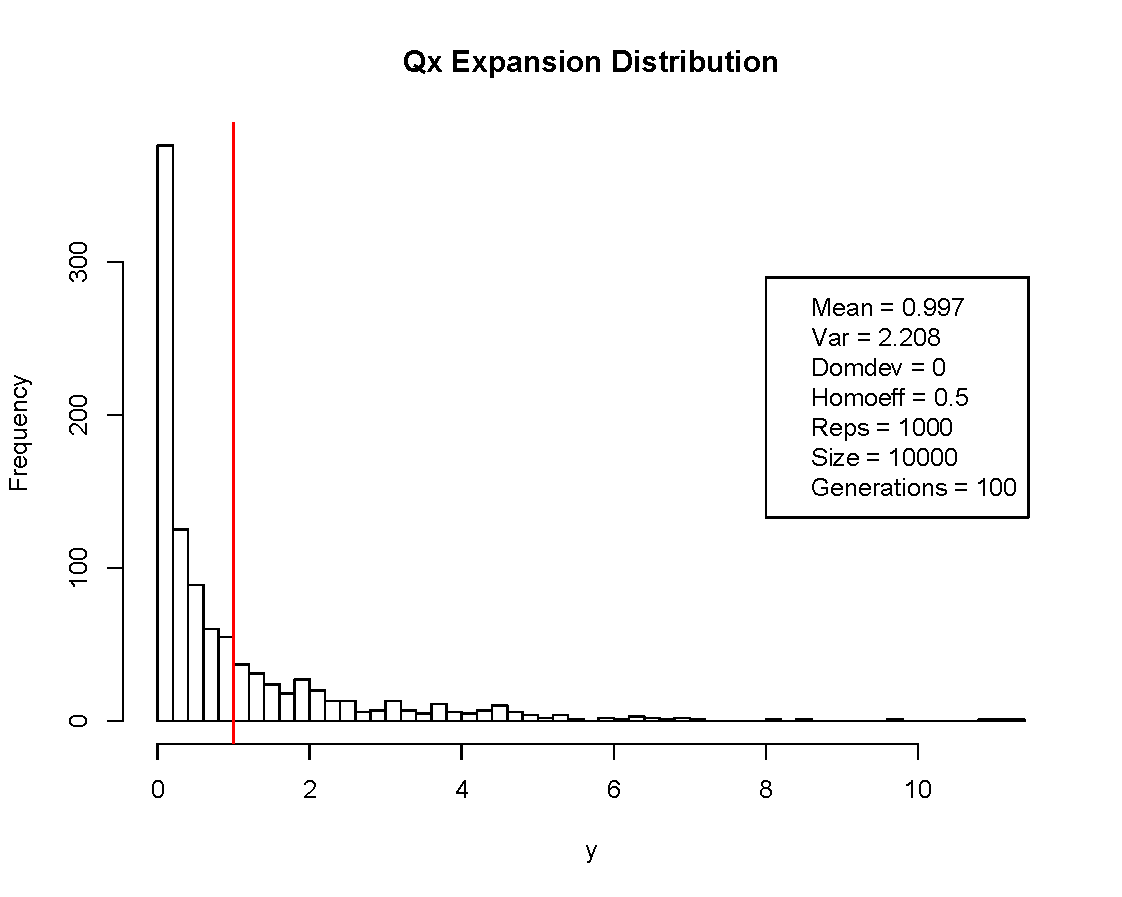
\includegraphics[width=80mm]{Qxexpdist} \caption*{Fig. 2: $Q_x$
      Expansion Distribution} \\
  \newline
  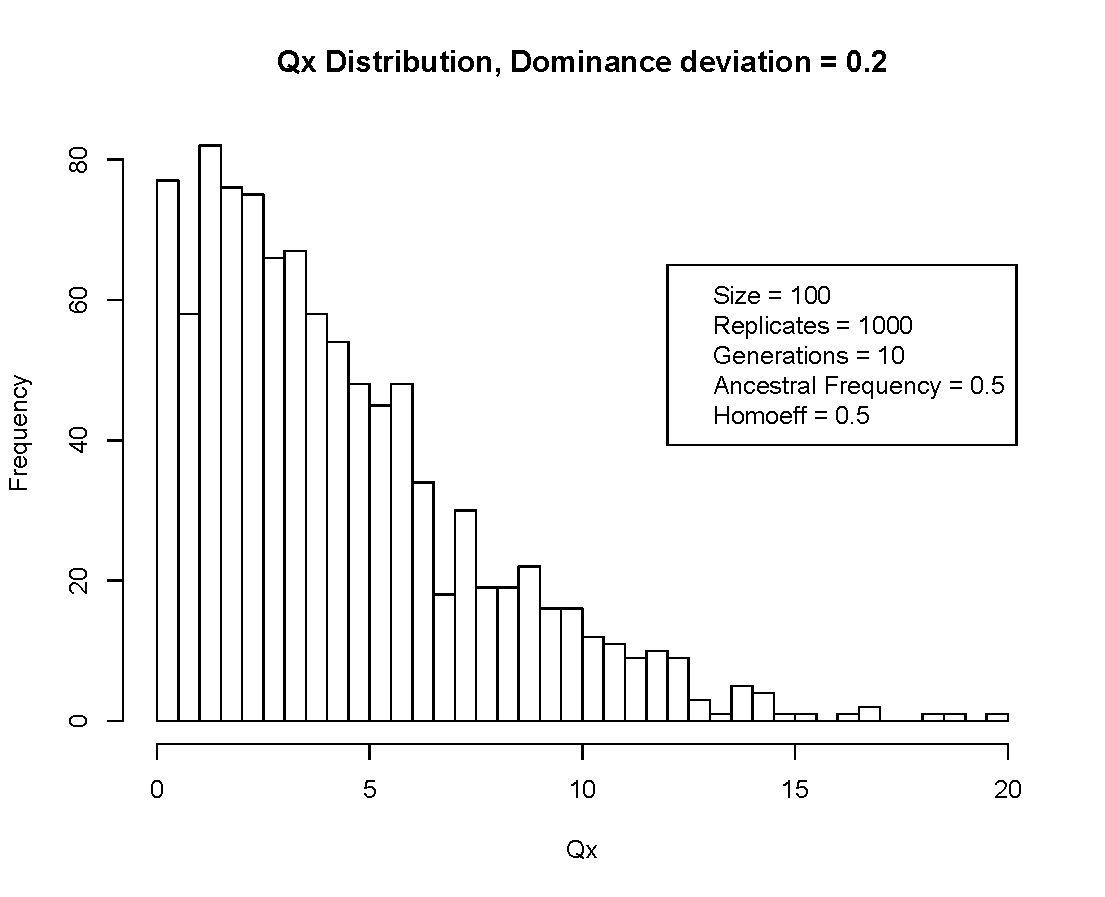
\includegraphics[width=80mm]{Qxdomdev}\caption*{Fig. 3: $Q_x$
   Distribution with dominance}
    &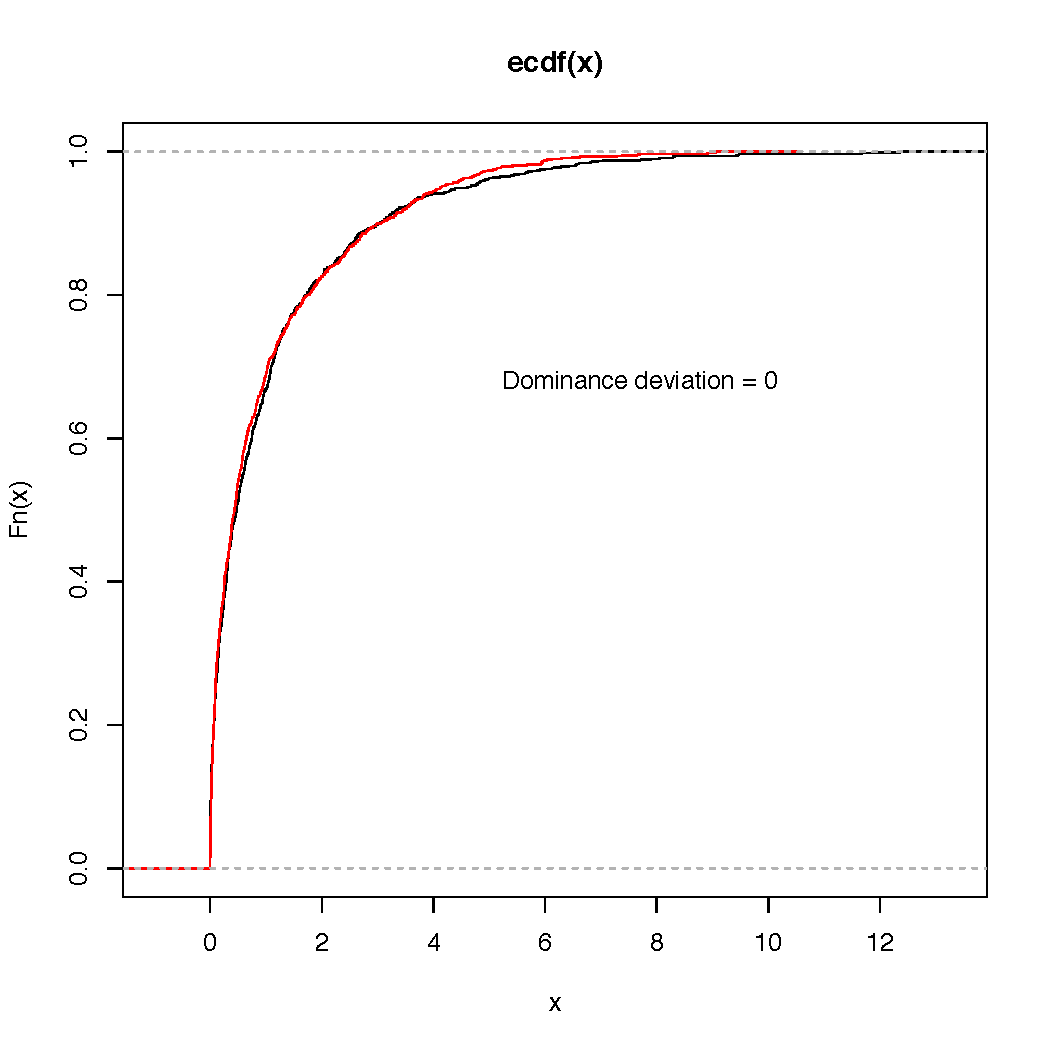
\includegraphics[width=80mm]{cdf0}\caption*{Fig. 4: Expected CDF
      of $Q_x$ with dominance = 0}\\
  \newline
  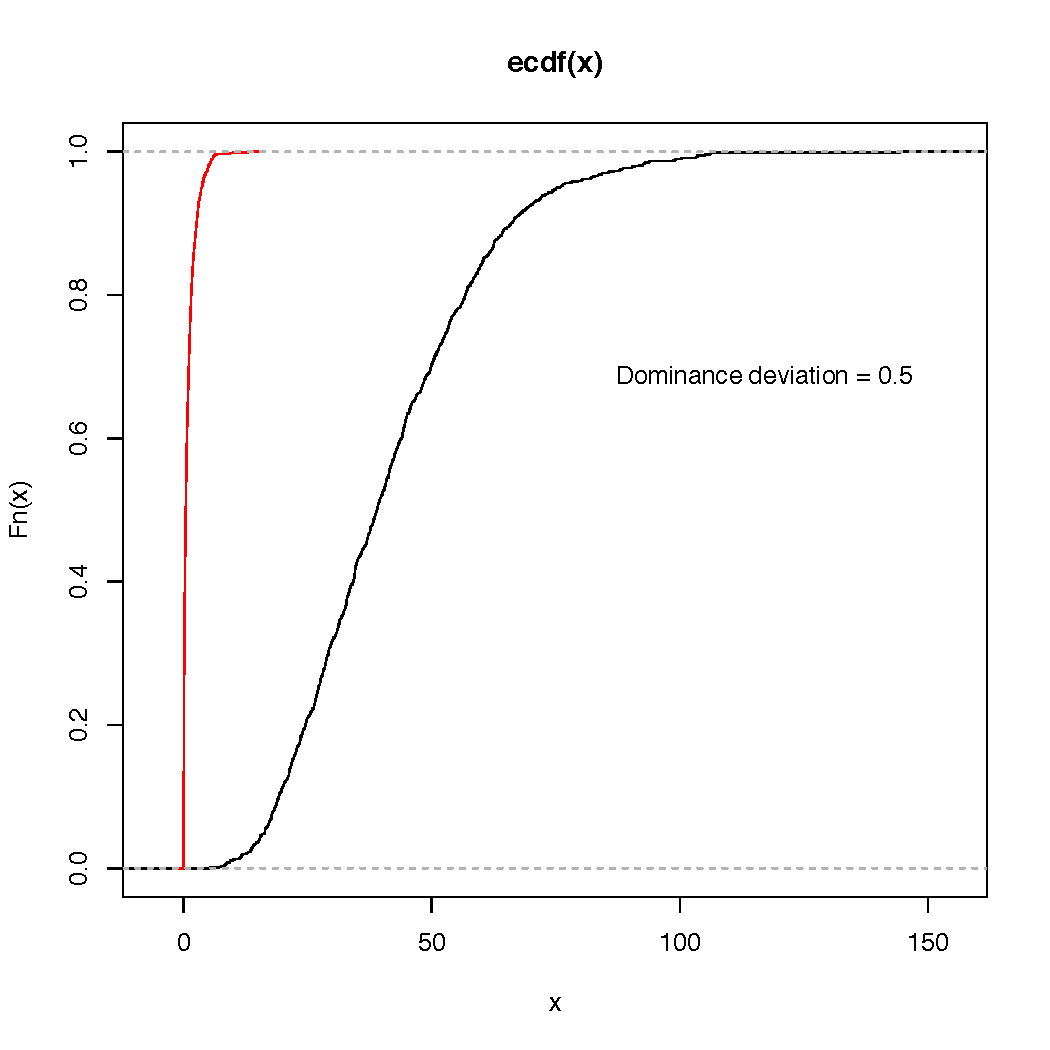
\includegraphics[width=80mm]{cdf05}\caption*{Fig. 5: $Q_x$
   Distribution with dominance = 0.5}
    &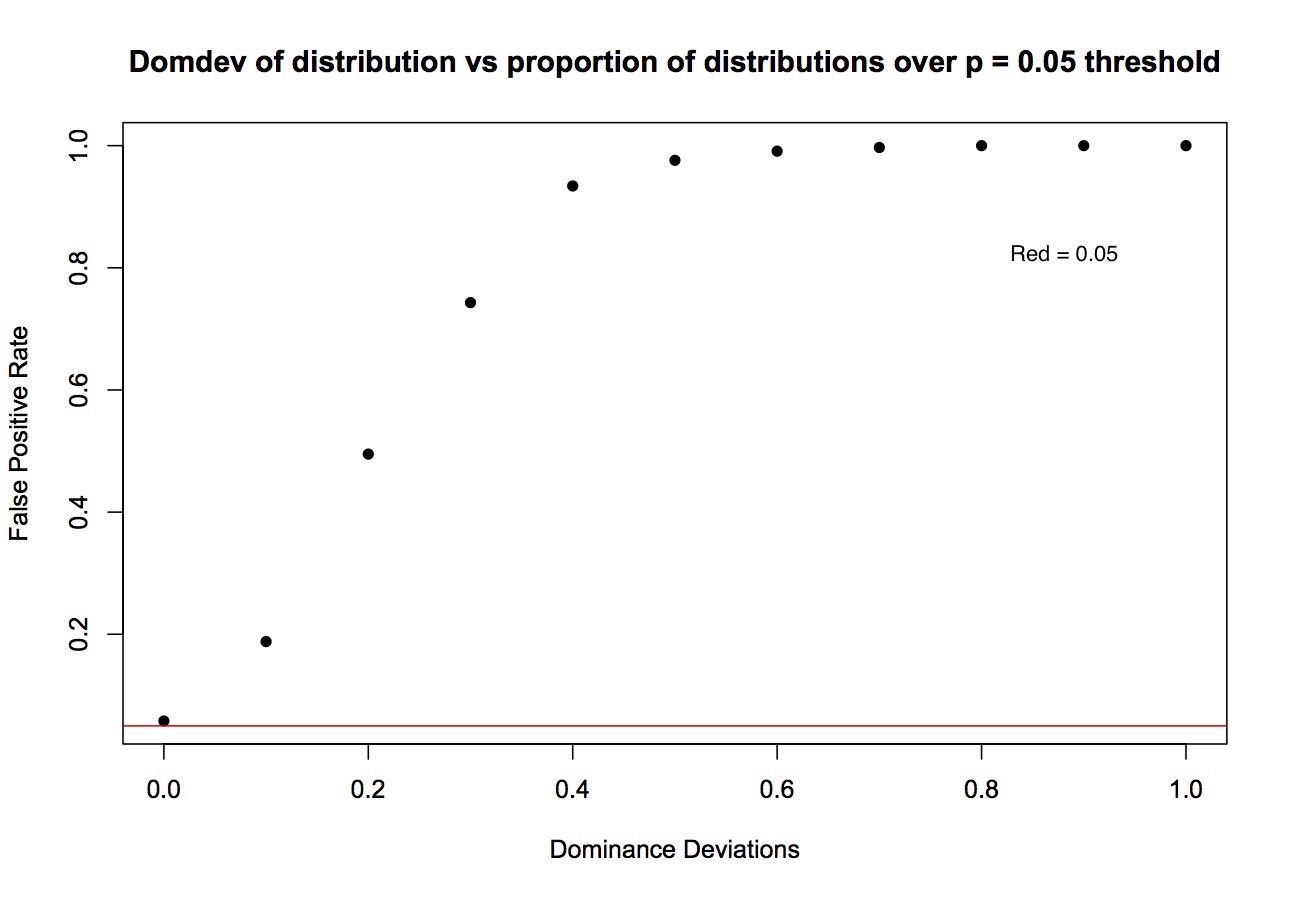
\includegraphics[width=80mm]{propover}\caption*{Fig. 6: Proportion
      of $Q_x$ over expected value for p = 0.5}\\
  \end{tabular}
 \end{table}

 \begin{table}[ht]
 \centering
 \begin{tabular}{ p{9cm}p{9cm} }
  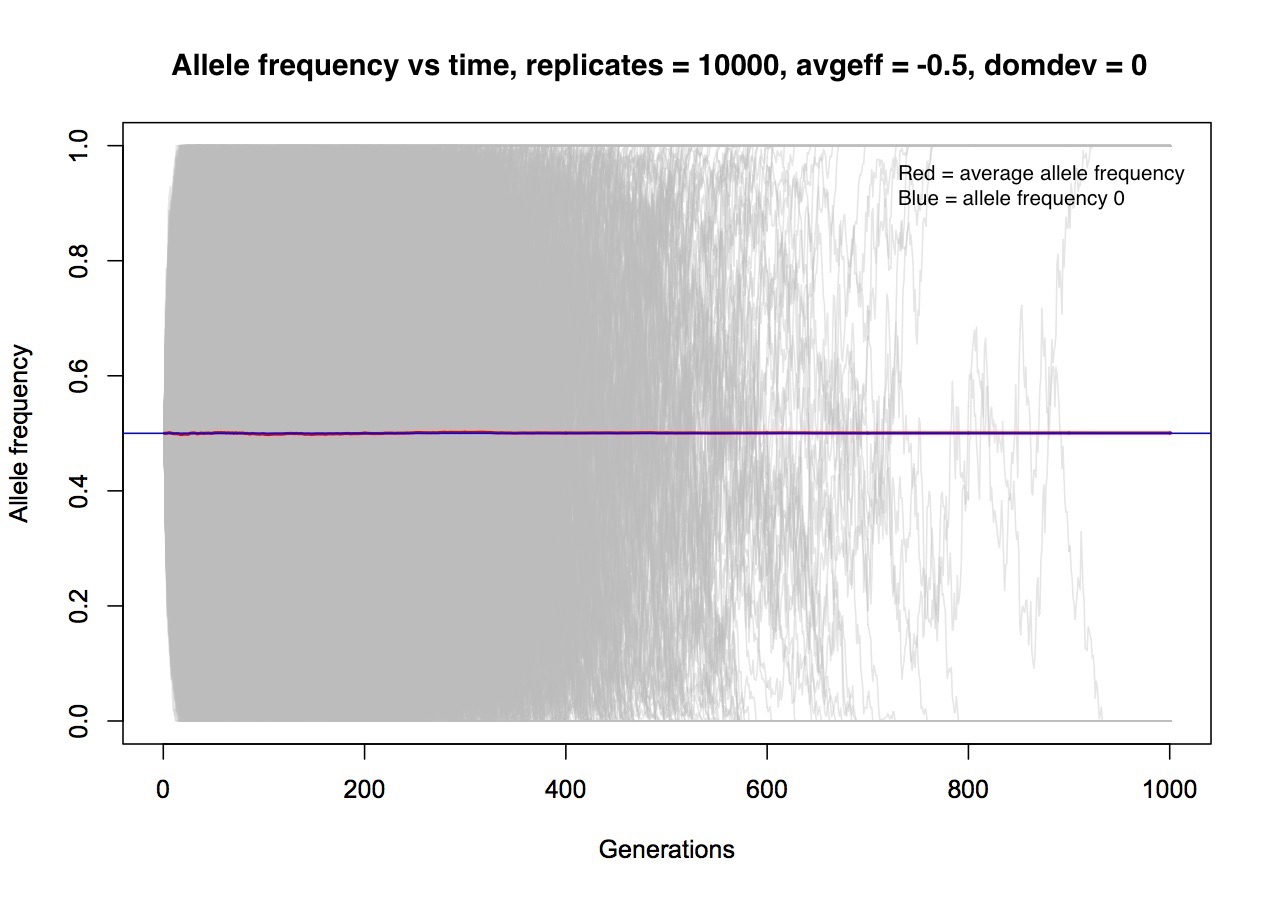
\includegraphics[width=80mm]{allelefreq0}\caption*{Fig. 7: Allele frequency over
   time for dominance = 0}
    &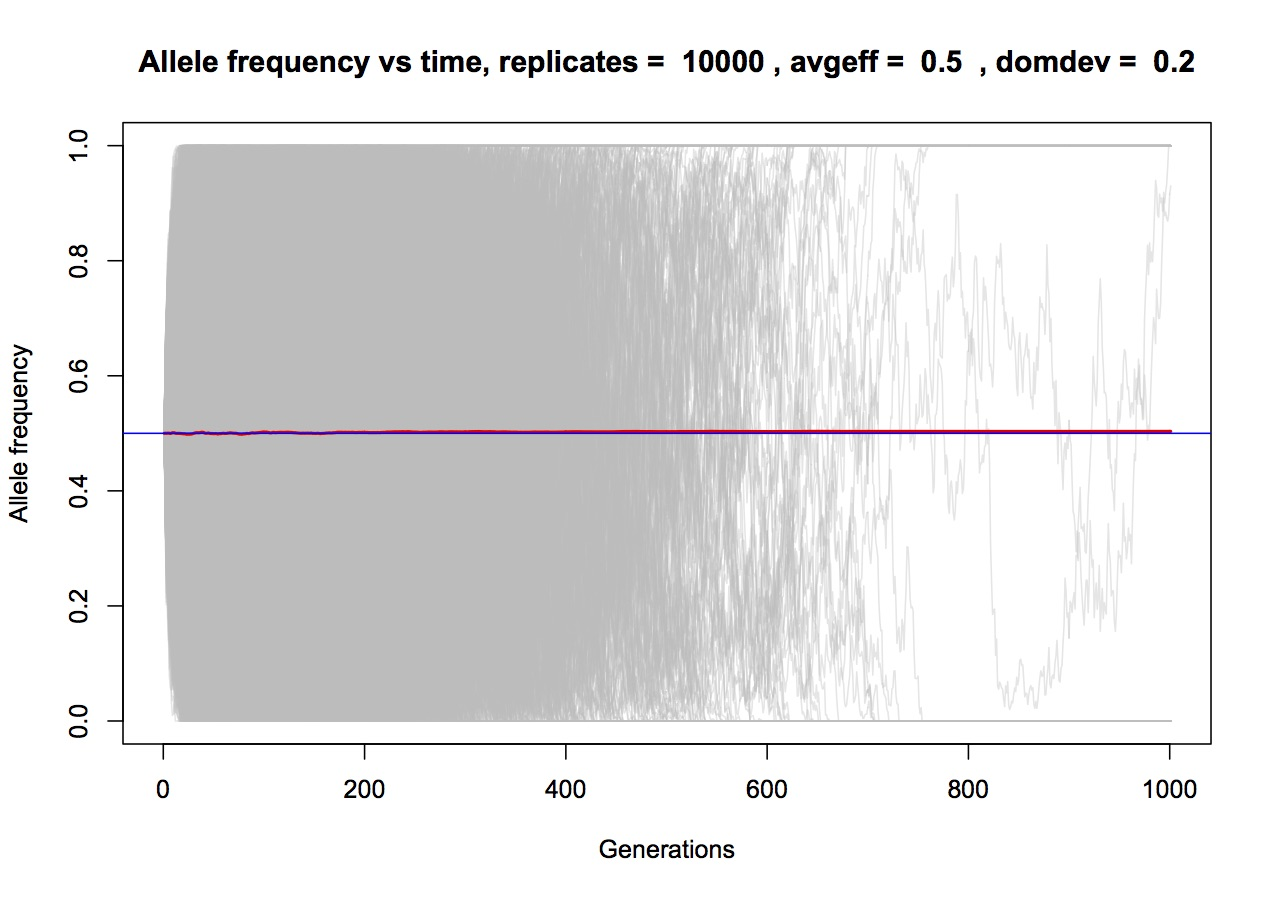
\includegraphics[width=80mm]{allelefreq02}\caption*{Fig. 8: Allele frequency over
   time for dominance = 0.2}\\
    \newline
  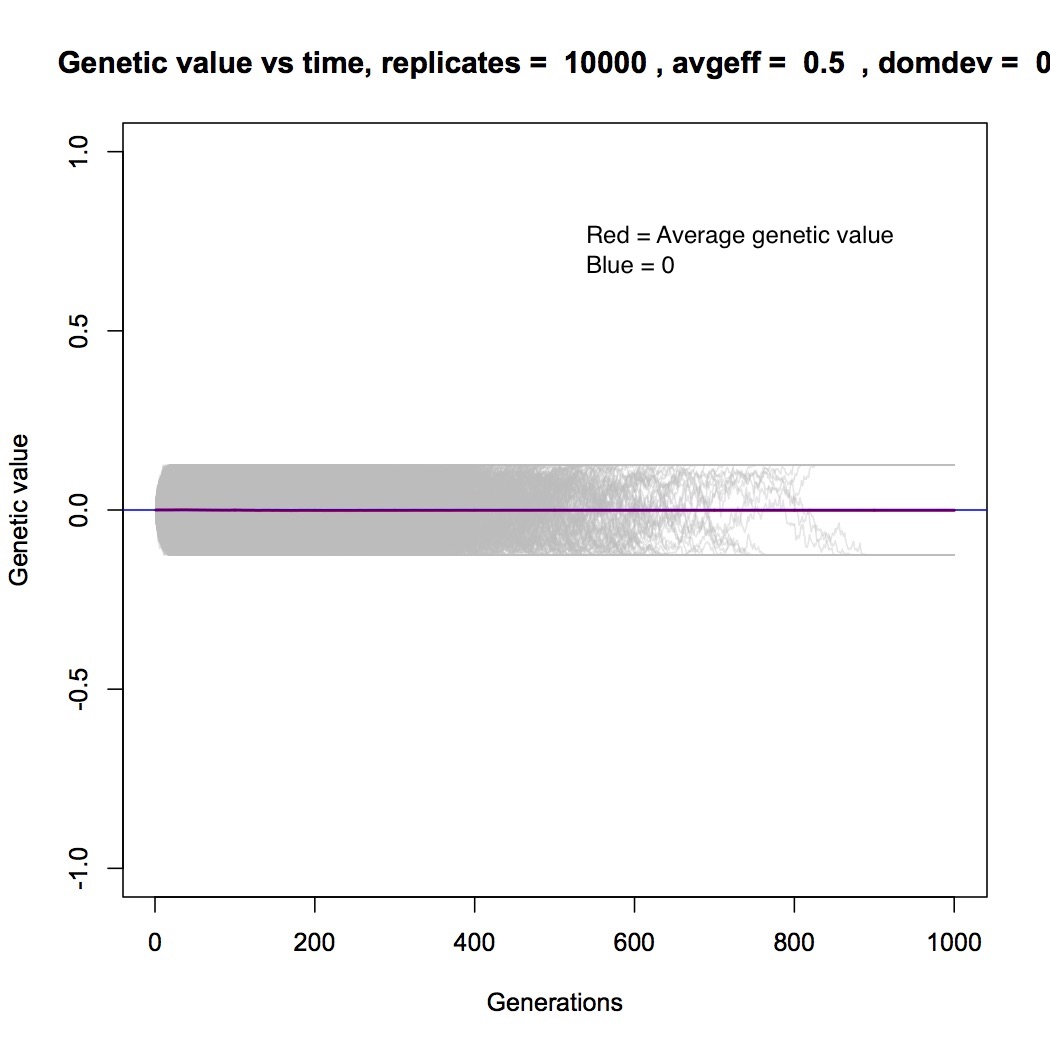
\includegraphics[width=80mm]{genval0}\caption*{Fig. 9: Genetic value
   over time for dominance = 0}
    &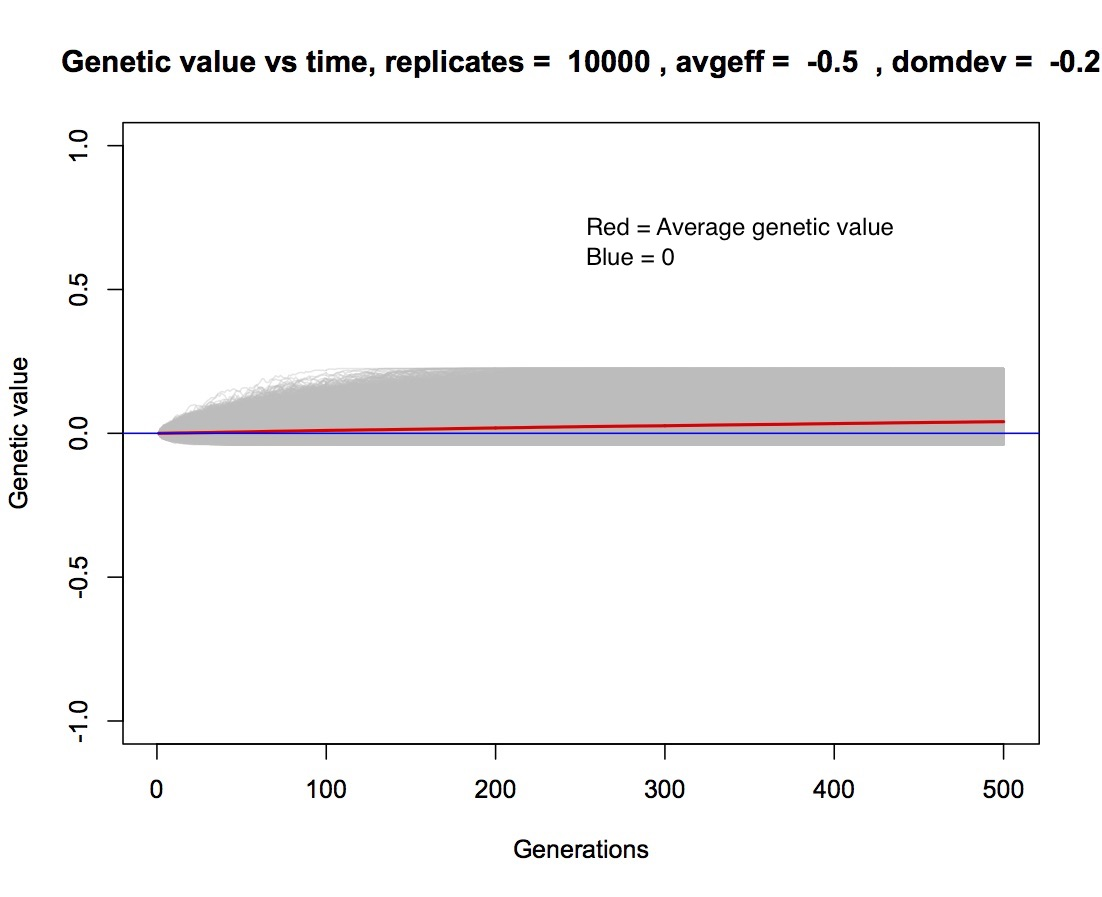
\includegraphics[width=80mm]{genval-02}\caption*{Fig. 10: Genetic value
      over time for dominance = -0.2}\\
    \newline
  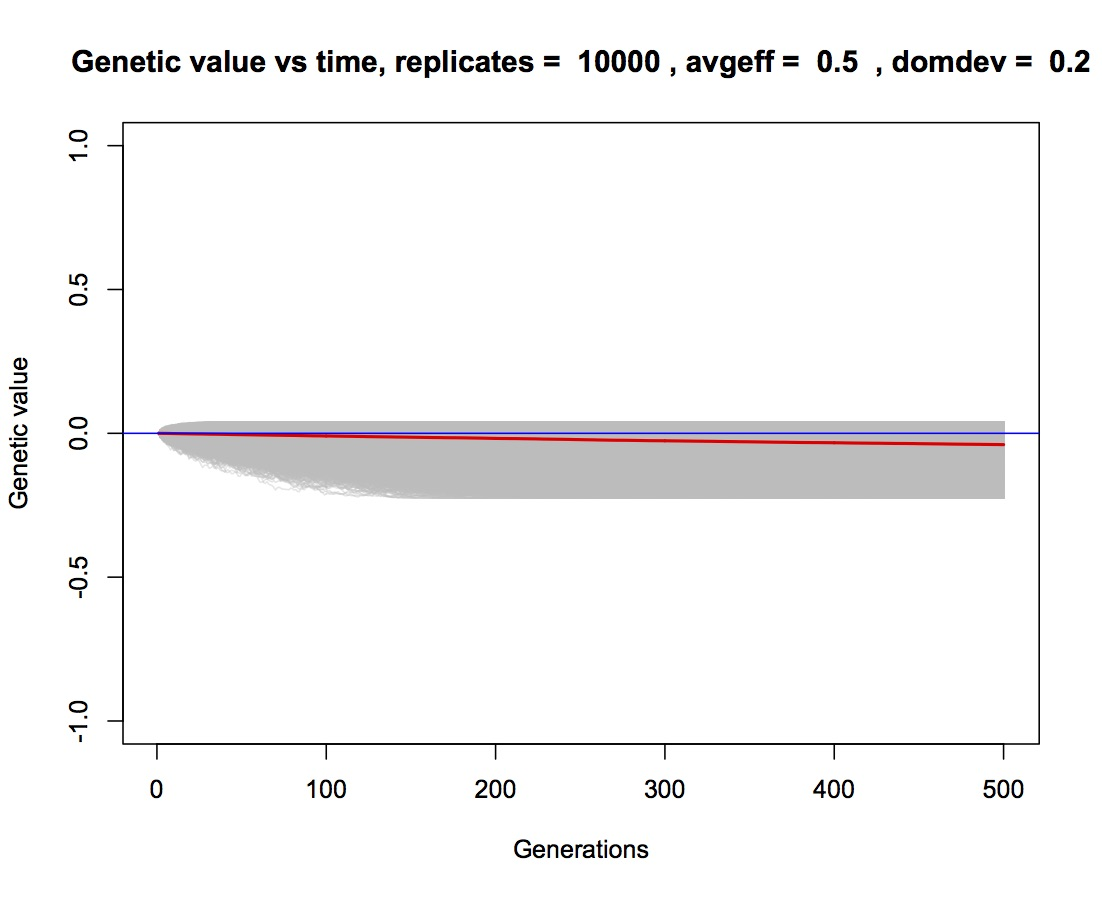
\includegraphics[width=80mm]{genval02}\caption*{Fig. 11: Genetic value
   over time for dominance = 0.2}
    &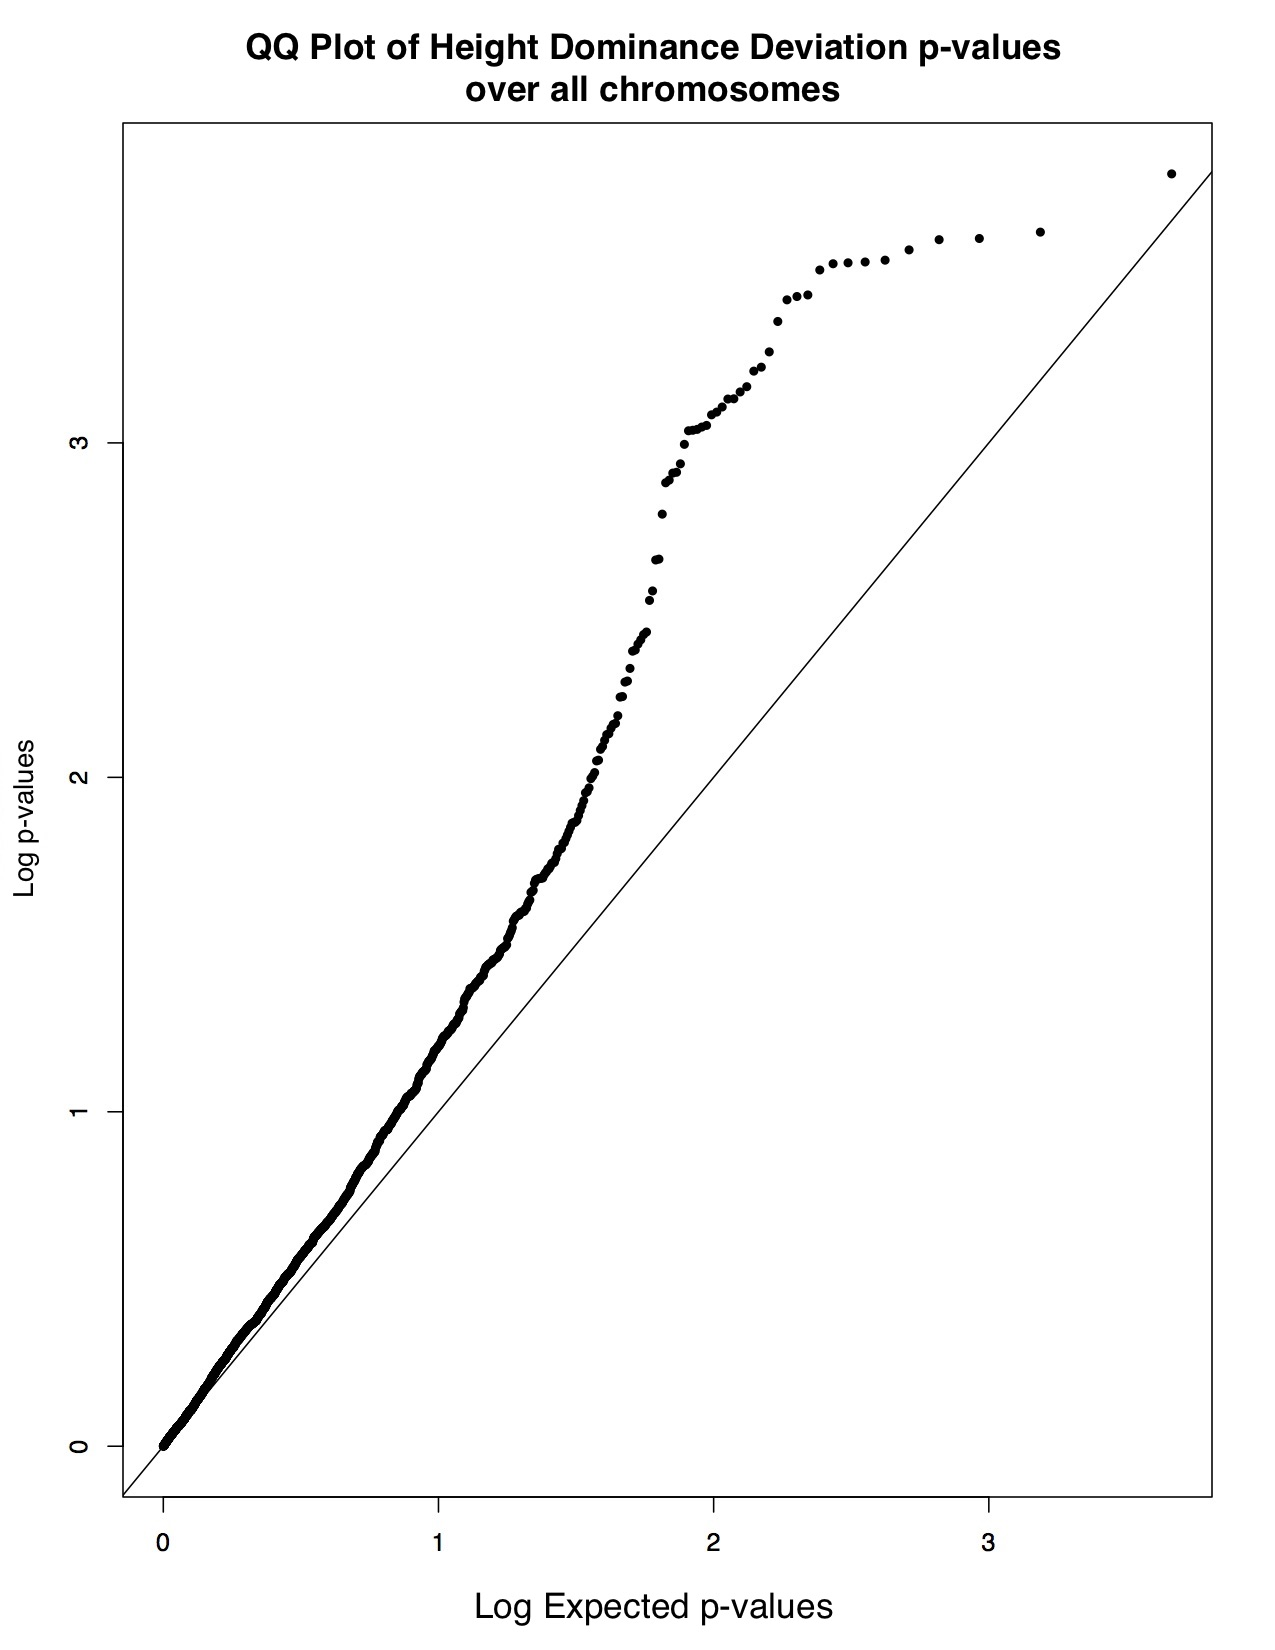
\includegraphics[width=70mm]{qqplot}\caption*{Fig. 12: Height
      Domiance Deviation p-value qqplot}
 \end{tabular}
 \end{table}

  \begin{table}[ht]
 \begin{tabular}{ p{9cm}p{9cm} }
  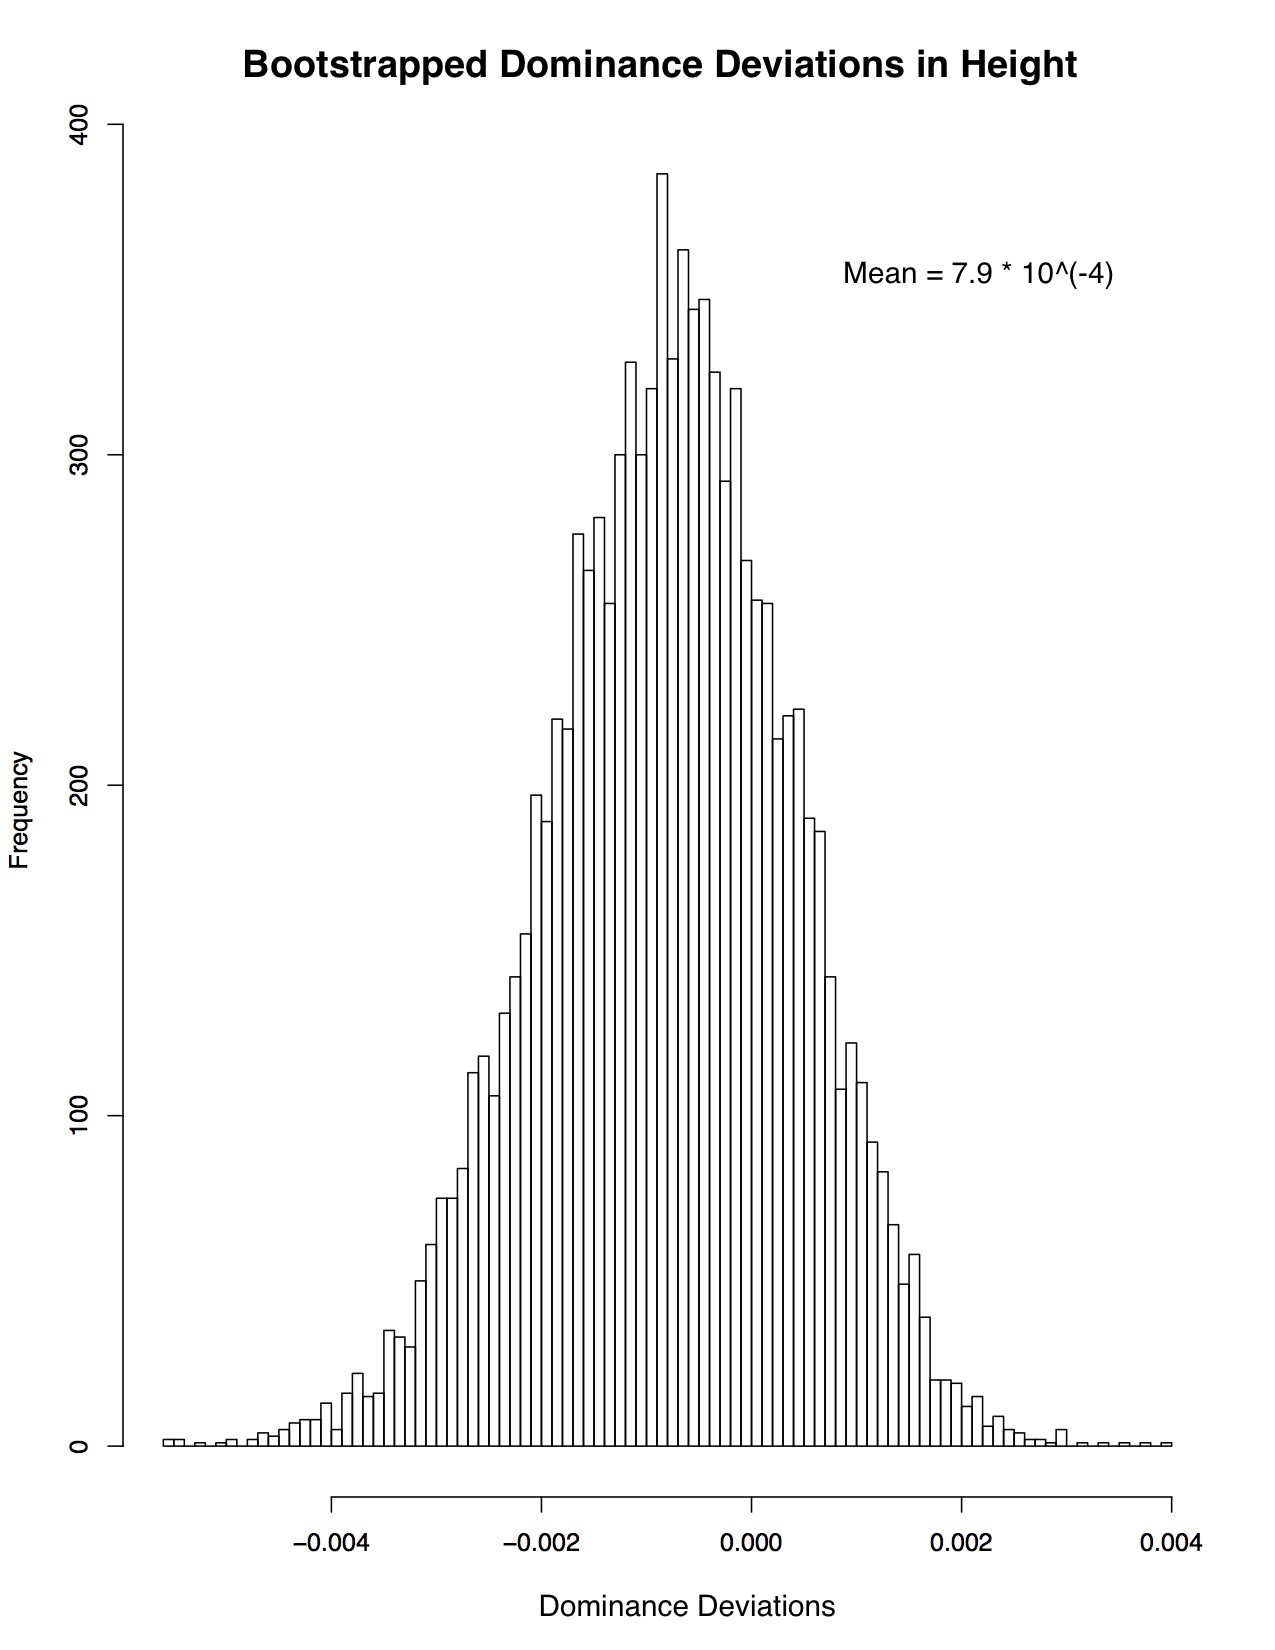
\includegraphics[width=80mm]{bootstrap}\caption*{Fig. 13:
   Bootstrapped Dominance Deviations for height for significant
   alleles}
 \end{tabular}
 \end{table}









\end{document}
